\documentclass{article}

\usepackage{babel}
\usepackage[letterpaper,top=2cm,bottom=2cm,left=2cm,right=2cm]{geometry}
\usepackage{amsmath}
\usepackage{amssymb}
\usepackage{graphicx}
\usepackage[colorlinks=true, allcolors=blue]{hyperref}
\setlength{\parindent}{0pt}

\title{Probing Biological Signal in DrugCLIP Protein Embeddings: A Case Study in Alzheimer's Disease}
\author{Eunice Chen, Muhaimen Shamsi, Dariia Kucheruk, Oleksii Nakhod}
\date{Milestone 2}

\begin{document}
\maketitle

\section*{Part I: Introduction and Background}

\subsection*{1. Research Question \& Significance}
Recent advances in contrastive learning have enabled the development of joint embedding spaces for proteins and small molecules. Models such as DrugCLIP \cite{adGwas2025,drugclipData2024} learn representations that align protein binding pockets with candidate ligands, enabling large-scale virtual screening without explicit molecular docking. This approach aligns with the growing need for precision drug development in Alzheimer's disease (AD) to address high clinical trial failure rates. However, it remains unclear to what extent these learned embeddings capture biologically meaningful structure beyond the specific objective they were trained on.

The goal of this project is to test the following hypothesis:

Do DrugCLIP protein embeddings encode biologically meaningful disease-related structure, specifically for Alzheimer's-associated proteins expressed in the hippocampus? \cite{adRegion2019,adRegion2022}

We investigate whether Alzheimer's-related proteins can be distinguished from other proteins using only their DrugCLIP embeddings. Rather than relying on unsupervised clustering, we frame this as a representation probing task: if a simple classifier trained on embedding vectors can reliably identify Alzheimer's-associated proteins, this would suggest that the embeddings contain latent disease-related information.

Understanding the biological content of learned molecular representations is important for AI-driven drug discovery \cite{adDrug2025}. Embedding models such as DrugCLIP are increasingly used as fast surrogates for binding prediction \cite{seaadPreprint2025} in virtual screening pipelines. If these representations encode biologically meaningful relationships among proteins, they could support additional tasks such as disease target prioritization, functional similarity search, and pathway-level analysis.

Our project focuses on evaluating the biological signal present in these representations through supervised learning, statistical testing, and embedding-space analysis.

\subsection*{2. Context \& Datasets}
DrugCLIP is a contrastive representation learning framework that maps protein binding pockets \cite{method2018} and small molecules into a shared embedding space. The model is trained on large-scale protein-ligand interaction data \cite{drugbank2018,chembl2019}, enabling rapid retrieval of candidate ligands using cosine similarity between embeddings.

Although the training objective focuses on protein-ligand compatibility, the resulting embeddings may implicitly encode structural or functional similarities among proteins. If this is the case, proteins associated with the same disease may occupy nearby regions in embedding space.

To test this hypothesis, we construct a dataset combining Alzheimer's disease annotations \cite{seaad2024} with brain-region expression data. The primary data sources include:
\begin{itemize}
    \item Allen Brain Atlas \cite{allenAtlas2012}: provides transcriptomic measurements across human brain regions. We use this dataset to identify genes expressed in the hippocampus, a region strongly affected in early Alzheimer's disease pathology.
    \item GWAS Catalog \cite{disgenet2023} and Alzheimer's genetic studies \cite{lambert2013}: provide lists of genes associated with Alzheimer's disease through genome-wide association studies and related genetic evidence.
    \item Protein structure databases (PDB \cite{pdb2000}): used for mapping protein names from GWAS-derived gene/protein lists.
    \item HGNC complete symbol mapping table \cite{hgncCompleteSet}: used to map gene symbols to UniProt accessions for embedding joins.
\end{itemize}

From these resources we construct a labeled dataset of proteins:
\begin{itemize}
    \item Positive class: proteins associated with Alzheimer's disease and expressed in the hippocampus.
    \item Negative class: proteins expressed in the hippocampus but not currently associated with Alzheimer's disease.
\end{itemize}
For each protein we retrieve a DrugCLIP embedding vector, which serves as the feature representation for downstream machine learning analysis.

\section*{Part II: Methods, Setup, and Results}

\subsection*{3. Methods}
Our objective is to determine whether Alzheimer's-related biological signal exists in DrugCLIP embeddings. We approach this as a representation evaluation problem using supervised classification and embedding-space analysis.

\subsubsection*{3.1 Embedding Retrieval}
For each protein in the dataset, we obtain structural models from the Protein Data Bank \cite{pdb2000}. Binding pockets are identified \cite{method2018} and encoded using the pretrained DrugCLIP protein encoder to produce dense embedding vectors. This results in a dataset $X \in \mathbb{R}^{N \times d}$, where $N$ is the number of proteins and $d$ is the embedding dimension. Each protein is associated with a binary label $y \in \{0,1\}$ indicating Alzheimer's association.

\subsubsection*{3.2 Classification Probe}
To test whether embeddings contain disease-related information, we train simple linear classifiers to predict Alzheimer's labels from embedding vectors.

Models considered include:
\begin{itemize}
    \item A linear probe on real DrugCLIP embeddings.
    \item A weighted binary cross-entropy variant to compensate for class imbalance.
    \item A random-embedding ablation.
    \item A label-shuffle ablation in which only the training labels are permuted.
\end{itemize}

We intentionally use simple models so that predictive performance reflects structure already present in the embeddings rather than complex nonlinear modeling. Performance is evaluated using 5-fold cross-validation with matched controls and repeated across two seeds in the current development-scale run.

\subsubsection*{3.3 Statistical Validation via Null Controls}
To confirm that classifier performance reflects meaningful signal rather than statistical artifacts, we compare the observed model against null controls.

The procedure is:
\begin{itemize}
    \item Shuffle Alzheimer's labels in the training fold while keeping the held-out test labels fixed.
    \item Replace embeddings with Gaussian noise for a representation-destruction control.
    \item Compare observed ROC-AUC and PR-AUC against these null runs.
\end{itemize}

This tests whether the model is learning a signal tied to the embeddings rather than exploiting trivial fold structure.

\subsubsection*{3.4 Embedding Geometry Analysis}
Beyond classification accuracy, we analyze the structure of the embedding space to determine whether disease proteins exhibit meaningful geometric organization.

\textbf{Distance structure test}
\begin{itemize}
    \item Compute pairwise cosine distances and compare AD--AD pairs versus AD--non-AD pairs.
    \item If embeddings encode biological similarity, AD--AD pairs should be significantly closer.
\end{itemize}

\textbf{Nearest-neighbor enrichment}
\begin{itemize}
    \item For each Alzheimer's protein, identify its $k$ nearest neighbors in embedding space.
    \item Measure enrichment for other Alzheimer's proteins and proteins involved in neurodegenerative pathways.
\end{itemize}

\subsubsection*{3.5 Visualization}
To visualize operating tradeoffs, we inspect mean ROC, precision-recall, and loss curves across seeds. These visualizations complement scalar metrics by showing where one model gains precision or recall relative to the null controls.

\subsection*{4. Data and Preprocessing}
Dataset construction proceeds as follows:
\begin{itemize}
    \item Collect Alzheimer's-associated genes from GWAS studies \cite{disgenet2023,lambert2013} and curated disease databases.
    \item Filter genes using Allen Brain Atlas expression data to retain those expressed in the hippocampus.
    \item Map genes to protein structures from PDB.
    \item Retrieve DrugCLIP embeddings for each protein.
\end{itemize}

Negative examples are sampled from hippocampus-expressed proteins that lack Alzheimer's disease annotations. Controls are matched within each fold at a ratio of two controls per AD gene, so the held-out positive prevalence is approximately $1/3$.

Model evaluation uses $k$-fold cross-validation, ensuring that proteins in test folds are never used during training. All preprocessing steps involving labels are performed within each fold to avoid information leakage.

\subsection*{5. Experimental Setup}
Primary evaluation metrics include:
\begin{itemize}
    \item ROC-AUC.
    \item PR-AUC.
    \item Accuracy.
\end{itemize}

The sampled multiseed dashboard reported here is curated under \texttt{documents/readme/ad\_predictor/}. This run contains 762 labeled samples total, with 254 AD positives and 508 matched controls, and reports 5-fold cross-validation averages over seeds 42 through 51.

\subsection*{6. Results}
The weighted binary cross-entropy model is the best-performing ablation in the current run, with mean test AUROC $= 0.545$ and mean test AUPRC $= 0.391$. The unweighted real-embedding probe is weaker (AUROC $= 0.533$, AUPRC $= 0.374$), while the two null-style controls stay near chance: random embedding reaches AUPRC $= 0.347$ and label shuffle reaches AUPRC $= 0.352$.

\begin{figure}[t]
    \centering
    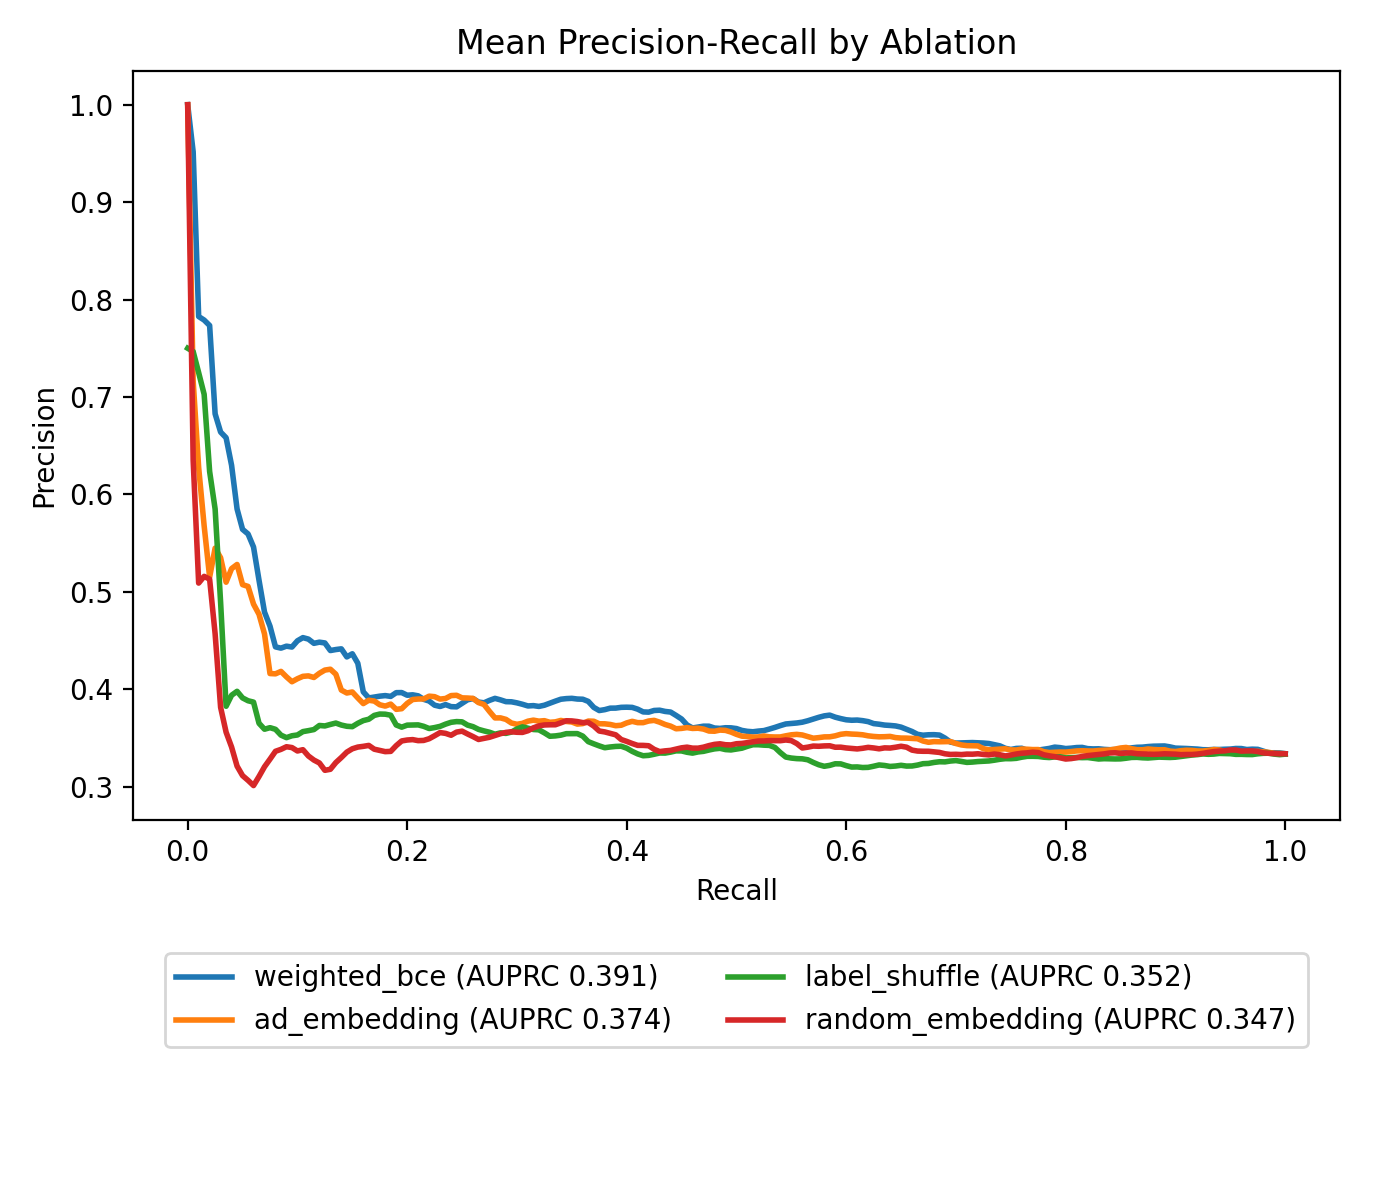
\includegraphics[width=0.48\linewidth]{../readme/ad_predictor/mean_auprc_by_ablation.png}
    \hfill
    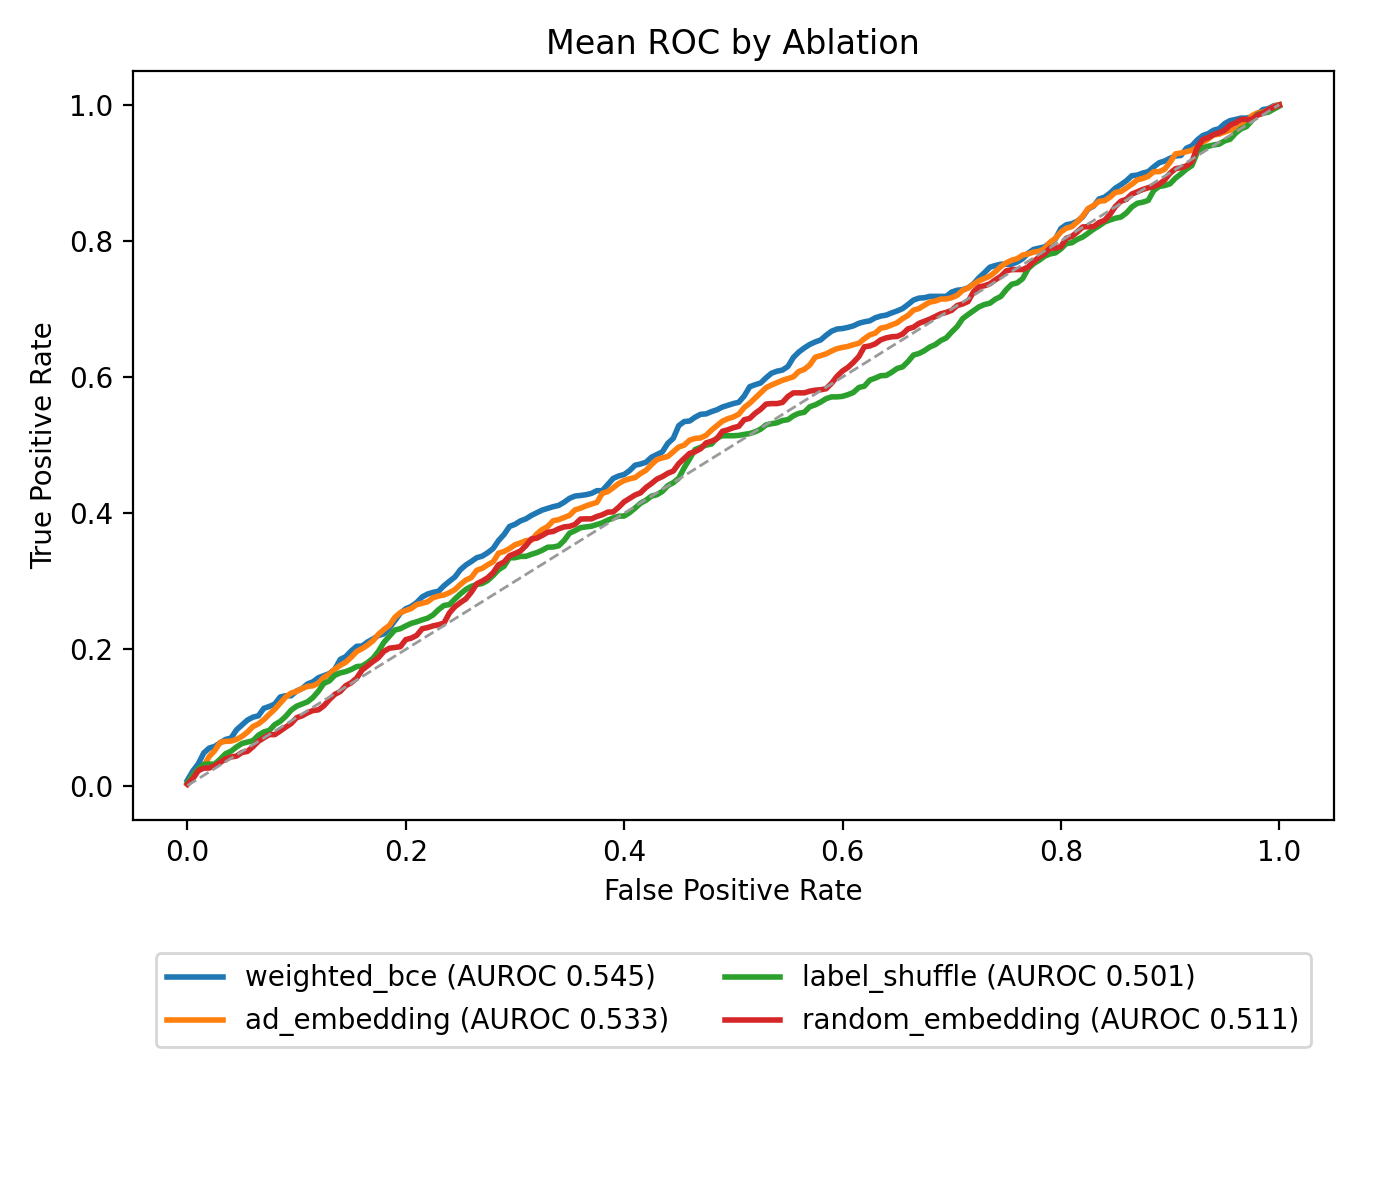
\includegraphics[width=0.48\linewidth]{../readme/ad_predictor/mean_auroc_by_ablation.png}
    \caption{Mean AUPRC and AUROC curves across ablations for the March 15, 2026 multiseed AD-predictor run. The AUPRC plot is the most informative view here because the positive prevalence is fixed at approximately one-third in the held-out matched-control test sets.}
\end{figure}

\begin{figure}[t]
    \centering
    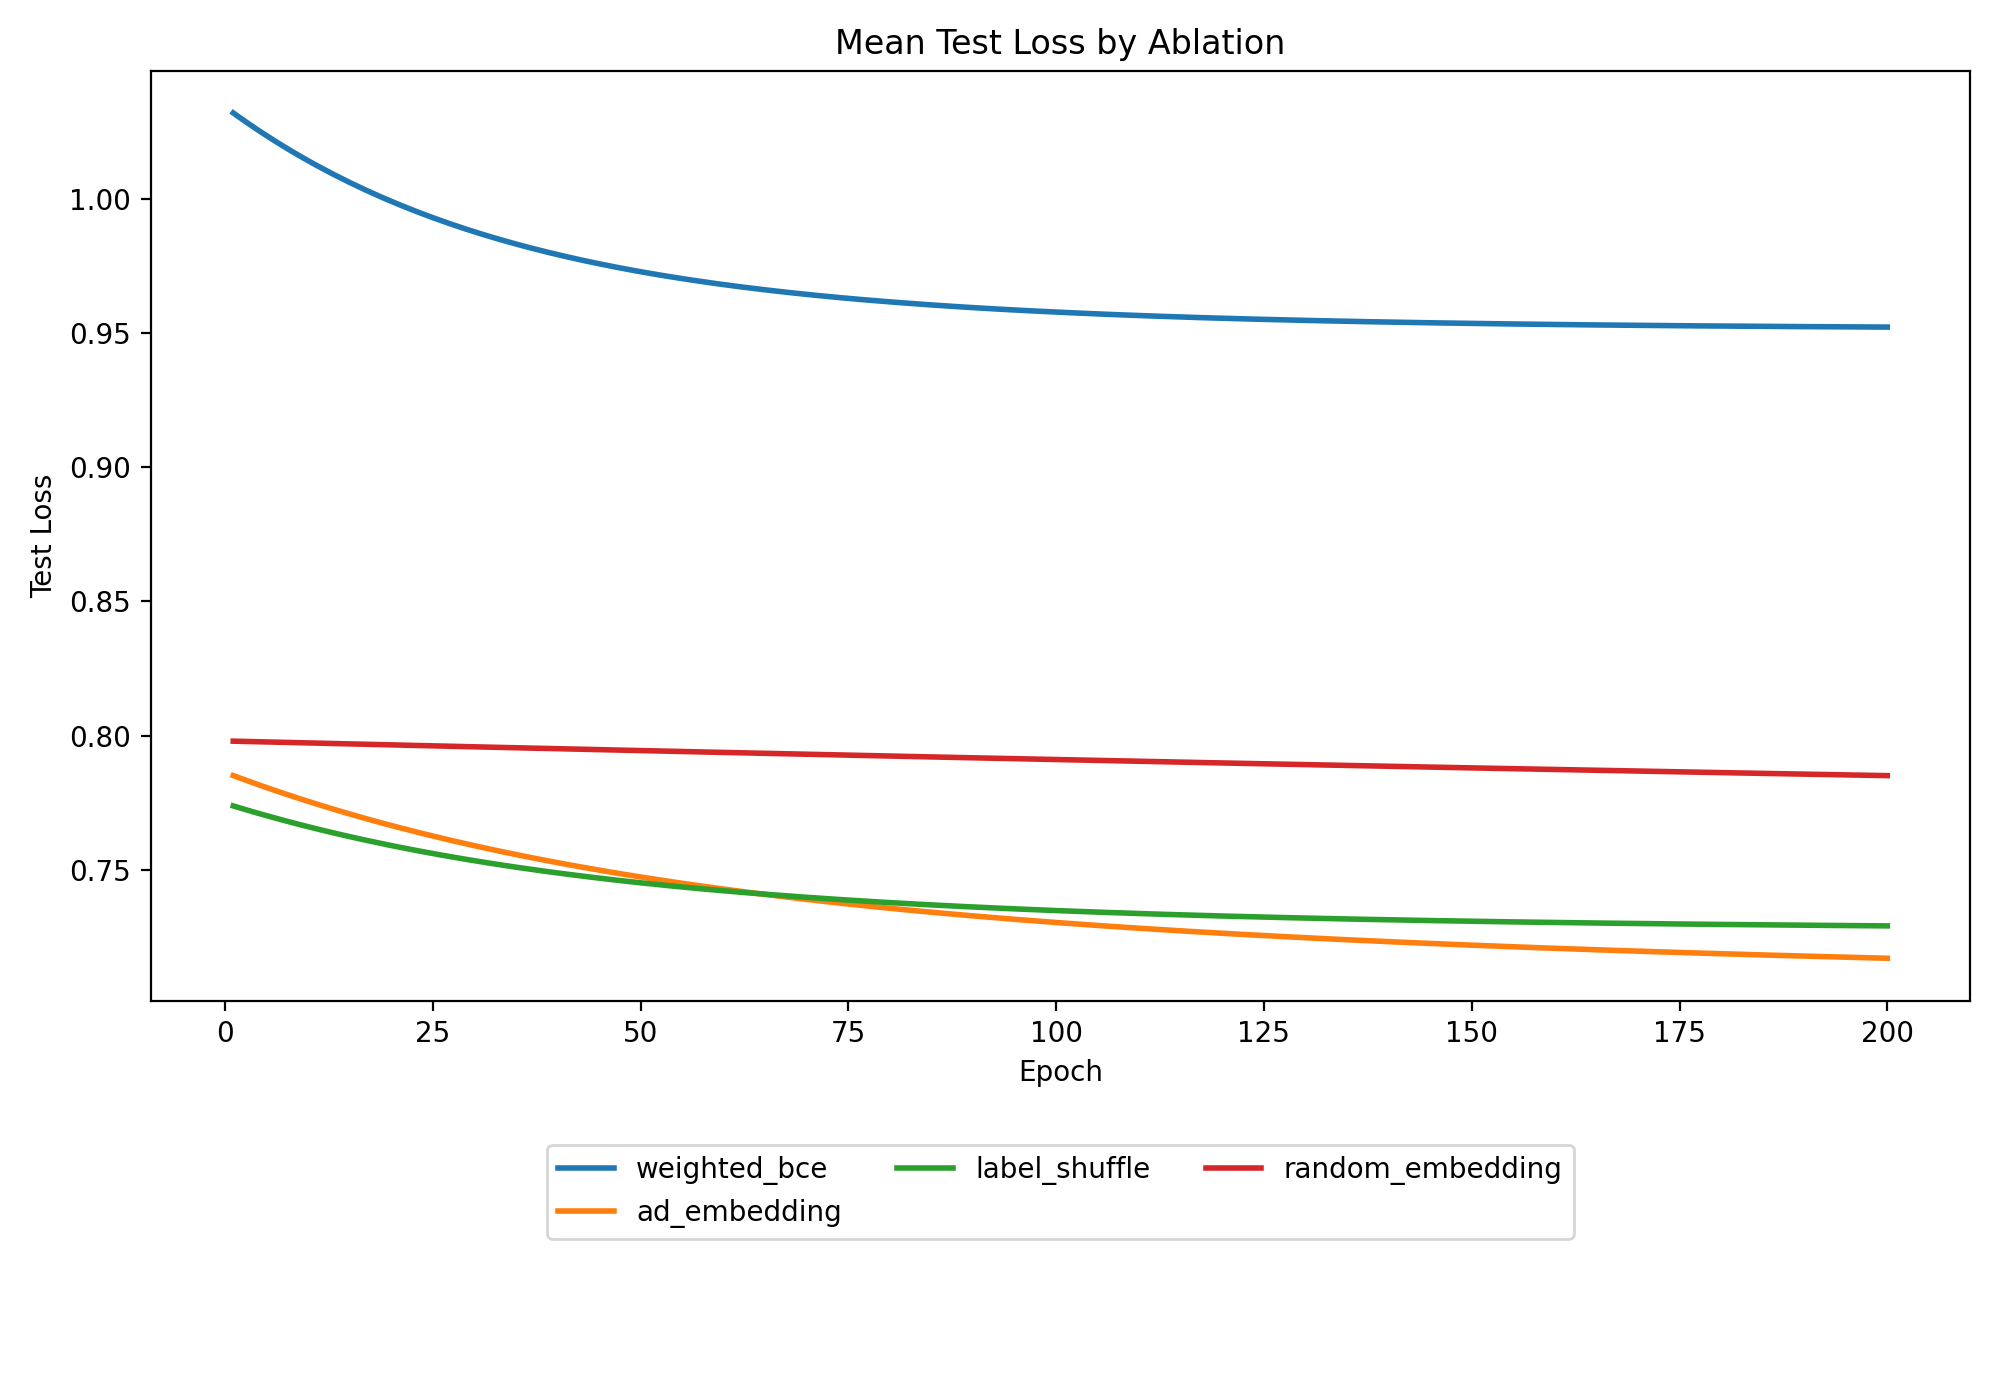
\includegraphics[width=0.7\linewidth]{../readme/ad_predictor/mean_test_loss_by_ablation.png}
    \caption{Mean test loss by ablation across the same multiseed run. The \texttt{ad\_embedding} curve is visibly lower than \texttt{random\_embedding}, but only slightly lower than \texttt{label\_shuffle}.}
\end{figure}

The precision-recall curves are particularly informative because the held-out test prevalence is fixed at approximately $0.333$. Under a no-skill ranking, the expected precision baseline is the positive prevalence \cite{varoquaux2023,martin2025}. The label-shuffle curve sits very close to that baseline, and its mean test AUPRC of $0.338$ is therefore consistent with a null model rather than a hidden predictive signal. This is useful diagnostically: it suggests the evaluation pipeline is not obtaining inflated PR performance from leakage or fold artifacts.

The curve shapes also show \emph{where} the observed model improves over the nulls. For the weighted-loss model, mean precision is about $0.450$ at recall $0.1$, versus $0.331$ for label shuffle and $0.338$ for random embeddings. At recall $0.3$, weighted BCE still maintains mean precision of about $0.386$, compared with $0.319$ for label shuffle and $0.363$ for random embeddings. This indicates that the main gain is not across the entire ranking uniformly; instead, the real-embedding model is concentrating more AD genes near the top of the ranked list, which is the practically important regime for target prioritization.

The ROC curves tell a similar but weaker story. At false-positive rate $0.2$, the weighted-loss model achieves mean true-positive rate $0.260$, compared with $0.191$ for label shuffle, $0.236$ for random embeddings, and $0.228$ for the unweighted real-embedding probe. This shows a real but modest separability advantage. At the same time, the full ROC curves remain fairly close to the diagonal, and even the best model only reaches mean true-positive rate $\approx 0.561$ at false-positive rate $0.5$. That pattern argues against a strong globally separable signal. The embedding appears to contain weak, distributed AD-related information, not a clean class boundary.

Comparing the two real-embedding variants suggests that class weighting mostly improves ranking quality in the early-retrieval regime rather than producing a dramatic change in overall discrimination. This is consistent with the dataset design: because the task uses matched controls and only moderate class imbalance, weighting is not rescuing a fundamentally broken classifier, but it does help move more positives into the top-scoring subset.

The mean test loss plot helps constrain the interpretation. Among the unweighted runs, the \texttt{ad\_embedding} curve sits clearly below \texttt{random\_embedding}, which is consistent with the real embeddings carrying more learnable structure than pure noise. At the same time, \texttt{ad\_embedding} is only modestly below \texttt{label\_shuffle}, so test loss is weaker evidence than the precision-recall curve for a specifically AD-aligned signal. Absolute loss values should not be compared directly across all ablations because weighted BCE rescales the objective.

Overall, the curves support a narrow claim: DrugCLIP embeddings contain a detectable but weak AD-related signal that is strongest in the top-ranked predictions and disappears under training-label permutation. The results support using the embedding as one component of a prioritization stack, but not as a standalone disease classifier.

\section*{Part III: Summary}
The current results are encouraging but still limited in scale. The real-embedding probe outperforms both null controls, and the precision-recall behavior is consistent with meaningful early enrichment rather than a purely random ranking. However, the small AUROC gain and the closeness of the null curves to the observed curve indicate that the signal is subtle. The next step is to combine this probe evidence with the independent network analyses and candidate-retrieval outputs so that no single weak metric carries the full biological claim.

\bibliographystyle{unsrturl}
\bibliography{milestone_2}

\end{document}
